\subsection{COMPARISON RELATIONS BETWEEN STRICTLY POSITIVE FUNCTIONS}

Let \(g\) be a function in \(\mathcal{H}(\mathfrak{F},\mathbf{R})\) which is strictly positive on a set in \(\mathfrak{F}\) . Comparison relations featuring \(g\) can be formulated in another way: the relation \(\mathbf{f} \preccurlyeq g\) is equivalent to saying that \(\| \mathbf{f}\| /g\) (which is defined on a set in \(\mathfrak{F}\) ) is bounded on a set in \(\mathfrak{F}\) ; the relation \(\mathbf{f} \ll g\) is equivalent to saying that \(\| \mathbf{f}\| /g\) tends to 0 along \(\mathfrak{F}\) . If \(f\) is a function in \(\mathcal{H}(\mathfrak{F},\mathbf{R})\) the relation \(f\asymp g\) means that \(f / g\) is logarithmically bounded on a set in \(\mathfrak{F}\) , and the relation \(f\sim g\) that \(f / g\) tends to 1 along \(\mathfrak{F}\) . If \(f\) is a function in \(\mathcal{H}(\mathfrak{F},\mathbf{R})\) and positive on a set in \(\mathfrak{F}\) , to say that \(f\) and \(g\) are comparable implies that \(f / g\) tends to a limit (finite or equal to \(+\infty\) ) along \(\mathfrak{F}\) .

PROPOSITION 9. Let \(f\) and \(g\) be two functions in \(\mathcal{H}(\mathfrak{F},\mathbf{R})\) , strictly positive on a set in \(\mathfrak{F}\) . For \(f\) and \(g\) to be comparable it is necessary and sufficient that for every number \(t \geqslant 0\) , with at most one exception, the function \(f - tg\) has constant sign \(^3\) on a set in \(\mathfrak{F}\) .

The condition is necessary. Indeed, if \(f \ll g\) one has \(f - tg \sim -tg\) except for \(t = 0\) , so \(f - tg\) is strictly negative on a set in \(\mathfrak{F}\) , except for \(t = 0\) ; if \(f \gg g\) then \(f - tg\) is strictly positive on a set in \(\mathfrak{F}\) for all \(t\) ; finally, if \(f \sim kg\) ( \(k\) constant \(> 0\) ), then \(f - tg \sim (k - t)g\) except for \(t = k\) , so, except perhaps for \(t = k\) , \(f - tg\) has the sign of \(k - t\) on a set in \(\mathfrak{F}\) .

The condition is sufficient. Indeed, suppose that the ratio \(f / g\) has two distinct cluster points \(\alpha < \beta\) along \(\mathfrak{F}\) . For every number \(t\) such that \(\alpha < t < \beta\) there then exist in every set \(X \in \mathfrak{F}\) two points \(x_{1}, x_{2}\) such that \(f(x_{1}) / g(x_{1}) < t\) and \(f(x_{2}) / g(x_{2}) > t\) ; thus \(f(x) - tg(x)\) does not have constant sign on \(X\) ; we have arrived at a conclusion incompatible with the hypothesis. It follows that \(f / g\) can have only one cluster value (finite or infinite) along the filter with base \(\mathfrak{F}\) , and consequently, (Gen.~Top., I, p.~85, corollary) has this value as its limit along \(\mathfrak{F}\) .

PROPOSITION 10. Let \(f\) and \(g\) be two functions in \(\mathcal{H}(\mathfrak{F},\mathbf{R})\) which are strictly positive on a set in \(\mathfrak{F}\) ; for every \(\alpha\) real and \(\neq 0\) the relation \(f\asymp g\) (resp. \(f\sim g\) ) is equivalent to \(f^{\alpha}\asymp g^{\alpha}\) (resp. \(f^{\alpha}\sim g^{\alpha}\) ); if \(\alpha >0\) the relation \(f\preccurlyeq g\) (resp. \(f\ll g\) ) is equivalent to \(f^{\alpha}\preccurlyeq g^{\alpha}\) (resp. \(f^{\alpha}\ll g^{\alpha}\) ); if \(\alpha < 0\) it is equivalent to \(f^{\alpha}\succcurlyeq g^{\alpha}\) (resp. \(f^{\alpha}\gg g^{\alpha}\) ).

The proofs are immediate.

One notes that in \(\mathcal{H}(\mathfrak{F},\mathbf{R})\) the set \(\varGamma\) of functions strictly positive on a set in F is such that \(\varGamma/\mathrm{R}_{\infty}\) is a multiplicative group \(\varGamma_{\infty}\) in \(\mathcal{H}_{\infty}(\mathfrak{F},\mathbf{R})\) ; \(\varGamma/\mathrm{R}_{0}\) is identical to the quotient group of \(\varGamma_{\infty}\) by the subgroup of classes (mod. \(R_{\infty}\) ) of logarithmically bounded functions in \(\varGamma\) ; on \(\varGamma/R_{0}\) the order relation deduced from the relation \(f \preccurlyeq g\) by passage to the quotient is compatible with the group structure of \(\varGamma/R_{0}\) and thus makes it an ordered group.

PROPOSITION 11. Let g be a function in \(\mathcal{H}(\mathfrak{F},\mathbf{R})\) such that \(\lim_{\mathfrak{F}}g = +\infty\) ; the relation \(f \ll g\) implies \(e^{f} \ll e^{g}\) ; the relation \(f \sim g\) implies \(\log f \sim \log g\) .

Indeed, if \(f \ll g\) then \(f - g = g\left(\frac{f}{g} - 1\right)\) tends to \(-\infty\) along \(\mathfrak{F}\) . Similarly, if \(f \sim g\) one has \(\log f = \log g + \log \frac{f}{g}\) , so \(\log f - \log g\) tends to 0, and the same for \(\frac{\log f}{\log g} - 1 = \frac{\log f - \log g}{\log g}\) .

\pandocbounded{
\includegraphics[keepaspectratio]{images/part002_2162bedd.jpg}}

On the other hand, note that the relation \(f \sim g\) does not imply \(e^{f} \sim e^{g}\) , nor even that \(e^{f} \asymp e^{g}\) , as is shown by the example where \(f(x) = x^{2}\) , \(g(x) = x^{2} + x\) as x tends to \(+\infty\) ; similarly, the relation \(f \ll g\) does not imply \(\log f \ll \log g\) , as is shown by the example \(f(x) = x\) , \(g(x) = x^{2}\) as x tends to \(+\infty\) .

DEFINITION 5. Let g be a function in \(\mathcal{H}(\mathfrak{F},\mathbf{R})\) , strictly positive on a set in F, and such that \(\lim_{\mathfrak{F}}g=0\) or \(\lim_{\mathfrak{F}}g=+\infty\) . One says that a function \(f\in\mathcal{H}(\mathfrak{F},\mathbf{R})\) is of order \(\rho\) (finite or infinite) relative to g if \(\lim_{\mathfrak{F}}\log(|f|)/\log g=\rho\) .

Note that if f is of order \(\rho\) relative to g then f is of order \(-\rho\) relative to 1/g; one therefore need treat only the case where \(g(x)\) tends to \(+\infty\) along F.

\pandocbounded{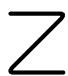
\includegraphics[keepaspectratio]{images/part002_5139c9a2.jpg}}

PROPOSITION 12. Let \(g\) be a function in \(\mathcal{H}(\mathfrak{F},\mathbf{R})\) such that \(\lim_{\mathfrak{F}}g = +\infty\) ; let \(f\) be a function in \(\mathcal{H}(\mathfrak{F},\mathbf{R})\) .

\begin{enumerate}
\def\labelenumi{\alph{enumi})}
\item
  For \(f\) to be of order \(+\infty\) relative to \(g\) it is necessary and sufficient that \(f \gg g^{\alpha}\) for every \(\alpha \geqslant 0\) .
\item
  For \(f\) to be of order \(-\infty\) relative to \(g\) it is necessary and sufficient that \(f \ll g^{-\alpha}\) for every \(\alpha > 0\) .
\item
  For \(f\) to be of finite order equal to \(\rho\) relative to \(g\) it is necessary and sufficient that, for every \(\varepsilon > 0\) , one has \(g^{\rho - \varepsilon} \ll f \ll g^{\rho + \varepsilon}\) .
\end{enumerate}

Let us prove c) for example. If the order of \(f\) relative to \(g\) is \(\rho\) then for every \(\varepsilon > 0\) there exists a set \(\mathbf{M} \in \mathfrak{F}\) such that, for every \(x \in \mathbf{M}\) , we have

\[
\left(\rho - \frac {\varepsilon}{2}\right) \log g (x) \leqslant \log | f (x) | \leqslant \left(\rho + \frac {\varepsilon}{2}\right) \log g (x),
\]

or \((g(x))^{\rho-\frac{\varepsilon}{2}} \leqslant |f(x)| \leqslant (g(x))^{\rho+\frac{\varepsilon}{2}}\) ; since \(\lim_{\mathfrak{F}} g = +\infty\) one thus has \(g^{\rho-\varepsilon} \ll f \ll g^{\rho+\varepsilon}\) for every \(\varepsilon > 0\) ; the converse is immediate. The proofs of a) and b) are similar.

Note that if \(f\) is of finite order \(\rho\) relative to \(g\) then \(fg^{-\rho}\) is of order 0 relative to \(g\) , and conversely; if \(f_1\) (resp. \(f_2\) ) is of order \(\rho_1\) (resp. \(\rho_2\) ) relative to \(g\) , and if \(\rho_1 + \rho_2\) is defined, then \(f_1f_2\) is of order \(\rho_1 + \rho_2\) relative to \(g\) .

Remarks. 1) Observe that though f may be of finite order \(\rho\) relative to g nevertheless the ratio \(f/g^{\rho}\) need not tend to a limit; for example, every logarithmically bounded function is of order 0 relative to g, but need not have a limit along F.

\begin{enumerate}
\def\labelenumi{\arabic{enumi})}
\setcounter{enumi}{1}
\tightlist
\item
  A function defined on a set in \(\mathfrak{F}\) need not have a determinate order (finite or not) relative to \(g\) , for the functions having a determinate order relative to \(g\) are comparable to all the powers of \(g\) with at most one exception. Now \(f\) need not have this property, as one sees from the example \(g(x) = x\) , \(f(x) = 1 + x^2 \sin^2 x\) (as \(x\) tends to \(+\infty\) ). In this example \(f\) is comparable to \(g^\alpha\) for \(\alpha < 0\) and \(\alpha > 2\) ; if one takes \(f(x) = e^x \sin^2 x + e^{-x} \cos^2 x\) then \(f\) is not comparable to any power (positive or negative) of \(g\) .
\end{enumerate}

